\documentclass[11pt, a4paper, twoside]{article}
% LTeX: language=es-AR

% Versión 1.er cuat 2021 Víctor Bettachini < vbettachini@unlam.edu.ar >

\usepackage[T1]{fontenc}
\usepackage[utf8]{inputenc}

\usepackage[spanish, es-tabla]{babel}
% \def\spanishoptions{argentina} % Was macht dass?
% \usepackage{babelbib}
% \selectbiblanguage{spanish}
% \addto\shorthandsspanish{\spanishdeactivate{~<>}}


\usepackage{graphicx}
\graphicspath{{./figuras/}{../LaTeX/}{../figurasLaTeX/}{./figs}}
% \usepackage{float}

\usepackage[arrowdel]{physics}
\newcommand{\pvec}[1]{\vec{#1}\mkern2mu\vphantom{#1}}
% \usepackage{units}
\usepackage[separate-uncertainty= true, multi-part-units= single, range-units= single, range-phrase= {~a~}, locale= FR]{siunitx}
\usepackage{isotope} % $\isotope[A][Z]{X}\to\isotope[A-4][Z-2]{Y}+\isotope[4][2]{\alpha}

\usepackage{tasks}
\usepackage[inline]{enumitem}
% \usepackage{enumerate}

\usepackage{hyperref}

% \usepackage{amsmath}
% \usepackage{amstext}
% \usepackage{amssymb}

\usepackage{tikz}
\usepackage{tikz-3dplot}
\usepackage{tikz-dimline}
\usetikzlibrary{calc}
% \usetikzlibrary{math}
\usetikzlibrary{arrows.meta}
\usetikzlibrary{snakes}
\usetikzlibrary{decorations}
\usetikzlibrary{decorations.pathmorphing}
\usetikzlibrary{patterns}

\usepackage[hmargin=1cm,vmargin=3cm, top= 0.75cm,nohead]{geometry}

\usepackage{lastpage}
\usepackage{fancyhdr}
\pagestyle{fancyplain}
\fancyhf{}
\setlength\headheight{28.7pt} 
\fancyhead[LE, LO]{\textbf{Mecánica Analítica Computacional} }
% \fancyhead[LE, LO]{\textbf{Mecánica General} }
\fancyhead[RE, RO]{\href{https://ingenieria.unlam.edu.ar/}{$\vcenter{\hbox{
\includegraphics[height=1cm]{ambos.pdf}}}$}}
\fancyfoot{\href{https://creativecommons.org/licenses/by-nc-sa/4.0/deed.es_ES}{$\vcenter{\hbox{
\includegraphics[height=0.4cm]{by-nc-sa_80x15.pdf}}}$} \href{https://ingenieria.unlam.edu.ar/}{DIIT - UNLaM}}
\fancyfoot[C]{ {\tiny Actualizado al \today} }
\fancyfoot[RO, LE]{Pág. \thepage/\pageref{LastPage}}
\renewcommand{\headrulewidth}{0pt}
\renewcommand{\footrulewidth}{0pt}

% LTeX: language = es-AR

\begin{document}
\begin{center}
  % \textsc{\large Mecánica general}\\
	\textsc{\large Vector posición}
	% \textsc{\large Vectores posición y velocidad. Energía cinética}
\end{center}
Debe poder resolver estos problemas en forma autónoma puede asumir que adquirió los conocimientos mínimos sobre los temas abordados.


\noindent
Genere un cuaderno Jupyter por ejercicio.
Para cada punto del mismo deberá usar al menos una celda de código.
Es buena práctica interponer otras celdas, pero de texto, en las que se indique de qué punto se trata.
 
\begin{enumerate}
% 	\section*{Vector posición}
	
	\item
		\begin{minipage}[t][10.5cm]{0.55\textwidth}
			\textbf{Posición suma}\\
			Realice los siguientes pasos definiendo las variables necesarias en \verb'SymPy' para que pueda verificar los resultados.
			\begin{enumerate}
				\item Guardar en una variable llamada \verb"a_r" un vector que indique la posición $\vec{r}_a = 3 \hat{e}_x + 0 \hat{e}_y + 5 \hat{e}_z$.
				En otra celda escriba \verb"a_r", y ejecute la celda para verificar que el vector fue guardado correctamente. 
				\item Guardar $\vec{r}_b = -5 \hat{e}_x + (-5) \hat{e}_y + 7 \hat{e}_z$ en \verb"b_r". Como en el paso anterior, verifique que el vector fue guardado correctamente.
				\item Restar las variables correspondientes para realizar $\Delta \vec{r}_{a \to b} = \vec{r}_b - \vec{r}_a$ y guardar el resultado en \verb"ab_deltaR".
				Verifique lo guardado.
				\item Guardar en \verb"c_r" (para el punto \verb"c", su posición \verb"r") el resultado de $\vec{r}_a +\Delta \vec{r}_{a \to b}$.
				Verifique.
				\item Para verificar que todo se hizo bien basta con leer \verb"c_r" y comprobar que $\vec{r}_c = \vec{r}_b$, para eso verifique el contenido de \verb"c_r".
			\end{enumerate}
		\end{minipage}
		\begin{minipage}[c][-4cm][t]{0.4\textwidth}
			% https://tex.stackexchange.com/questions/117140/easiest-way-to-draw-a-3d-coordinate-system-with-axis-labels-and-ticks-in-tikz
			\begin{tikzpicture}[x=0.5cm,y=0.5cm,z=0.3cm, scale=0.85]
				% The axes
				\draw[-LaTeX] (xyz cs:x=-8.5) -- (xyz cs:x=8.5) node[above] {$x$};
				\draw[-LaTeX] (xyz cs:y=-5.5) -- (xyz cs:y=8.5) node[right] {$z$};
				\draw[-LaTeX] (xyz cs:z=-8.5) -- (xyz cs:z=8.5) node[right] {$y$};
				% The thin ticks
				\foreach \cooZ in {-5,-4,...,8} {
					\draw (-1.5pt,\cooZ) -- (1.5pt,\cooZ);
				}
				\foreach \coo in {-8,-7,...,8}
				{
					\draw (\coo,-1.5pt) -- (\coo,1.5pt);
					\draw (xyz cs:y=-0.15pt,z=\coo) -- (xyz cs:y=0.15pt,z=\coo);
				}
				% The thick ticks
				\foreach \coo in {-5,5}
				{
					\draw[thick] (\coo,-3pt) -- (\coo,3pt) node[below=6pt] {\coo};
					\draw[thick] (-3pt,\coo) -- (3pt,\coo) node[left=6pt] {\coo};
					\draw[thick] (xyz cs:y=-0.3pt,z=\coo) -- (xyz cs:y=0.3pt,z=\coo) node[below=8pt] {\coo};
				}
				% base of versors
				\coordinate (O) at (0,0,0);
				\draw[thick,blue,-LaTeX] (O) -- (1,0,0) node[anchor=north]{$\hat{e}_x$};
				\draw[thick,blue,-LaTeX] (O) -- (0,0,1) node[anchor=west]{$\hat{e}_y$};
				\draw[thick,blue,-LaTeX] (O) -- (0,1,0) node[anchor=east]{$\hat{e}_z$};
				% Dashed lines for the points
				\draw[dashed]
				(xyz cs:z=-5) --
				+(0,7) coordinate (u) --
				(xyz cs:y=7) --
				+(-5,0) --
				++(xyz cs:x=-5,z=-5) coordinate (v) --
				+(0,-7) coordinate (w) --
				cycle;
				\draw[dashed] (u) -- (v);
				\draw[dashed] (-5,7) -- (-5,0) -- (w);
				\draw[dashed] (3,0) |- (0,5);
				% Dots and labels for
				\coordinate (a) at (3,5);
				\coordinate (b) at (v);
				\node[fill,circle,inner sep=1.5pt,label={above right:$(3,0,5)$}] at (a) {};
				\node[fill,circle,inner sep=1.5pt,label={above right:$(-5,-5,7)$}] at (b) {};
				\draw[red,-LaTeX] (O) -- (a) node [midway, above, left]{$\vec{r}_a$};
				\draw[red,-LaTeX] (O) -- (b) node [midway, below]{$\vec{r}_b$};
				% % The origin
				% \node[align=center] at (3,-3) (ori) {(0,0,0)\\\text{origen}};
				% \draw[-LaTeX,help lines] (ori) .. controls (1,-2) and (1.2,-1.5) .. (0,0,0);
			\end{tikzpicture}
		\end{minipage}


	\item
		\begin{minipage}[t][6cm]{0.68\textwidth}
			(*) \textbf{Vectores en función de una variable}\\
			Una partícula de masa \(m\) está engarzada en un aro de radio $R$, por lo que su radio medido desde el centro del aro es constante.
			Basta entonces conocer el ángulo $\varphi$ para describir su posición.
			\begin{enumerate}
				\item \textbf{Vector posición}\\
				Escríbalo en coordenadas cartesianas en función de \(R\) y \(\varphi\).
				Recuerde que la primera es constante, no es más que un símbolo para la biblioteca \verb'SymPy', en tanto que la segunda es una variable que depende del tiempo, o dinámica, en el léxico de la biblioteca.
				Evidentemente, deberá recurrir a funciones trigonométricas.
				Busque como estas se implementan en la biblioteca.
				\item \textbf{Velocidad}\\
				Haga que \verb'SymPy' calcule la velocidad en este sistema de referencia.\\
			Resultado:\\
				\(
					-  R \sin{\left(\varphi \right)} \dot{\varphi}\mathbf{\hat{e}_x} + R \cos{\left(\varphi \right)} \dot{\varphi}\mathbf{\hat{e}_y}
				\)
			\end{enumerate}
		\end{minipage}
		\begin{minipage}[c][-1.5cm][t]{0.15\textwidth}
			\begin{tikzpicture}[x=0.5cm,y=0.5cm,z=0.3cm, scale=1]
				% The axes
				\draw [-LaTeX] (0,0) -- (5,0) node[above] {$x$};
				\draw [-LaTeX] (0,0) -- (0,5) node[right] {$y$};
				\draw [very thick] (0,0) circle [radius= 4];
				\draw [-LaTeX, dashed] (1,0) arc [radius=1, start angle=0, end angle=300] node[midway,left] {$\varphi$};
				\draw [dashed] (0,0) -- ($(0,0)+(-60:4)$) node [midway,right] {$R$}; 
				\shade [ball color=black!80] ($(0,0)+(-60:4)$) circle(0.5) node [] {\color{white} $m$};
			\end{tikzpicture}
		\end{minipage}


%
%	\section*{Energía cinética}
%
%		\item
%		\begin{minipage}[t][5cm]{0.6\textwidth}
%			\textbf{Péndulo con punto de suspensión libre} [Landau \S5 ej. 2]\\
%			La partícula de masa \(m_2\) pende de una barra rígida de longitud \(\ell\) de masa despreciable.
%			El otro extremo de la misma está engarzada a una barra rígida dispuesta a lo largo del eje \(\hat{x}\).
%			El dispositivo de engarze tiene una  masa \(m_1\).\\
%			Exprese la energía cinética del sistema en función de las coordenadas indicadas por la figura: \(x, \phi\).
%		\end{minipage}
%		\begin{minipage}[c][1cm][t]{0.35\textwidth}
%			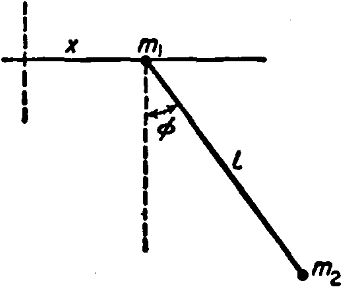
\includegraphics[width=\textwidth]{landauS52_fig2.png}
%		\end{minipage}
%
%
%		\item
%			\begin{minipage}[t][3cm]{0.7\textwidth}
%				\textbf{Péndulo doble} [Landau \S5 ej. 1]\\
%				Una barra rígida de longitud \(\ell_1\) tiene una masa despreciable respecto a la de la partícula de masa \(m_1\) fija a su extremo.
%				A su vez de esta última pende otra barra rígida, de longitud \(\ell_2\) que en su extremo tiene otra partícula de masa \(m_2\), también mucho mayor que aquella de la barra.\\
%				Exprese la energía cinética de este sistema en función de las coordenadas indicadas en la figura: \(\phi_1, \phi_2\).\\
%			\end{minipage}
%			\begin{minipage}[c][0.5cm][t]{0.3\textwidth}
%				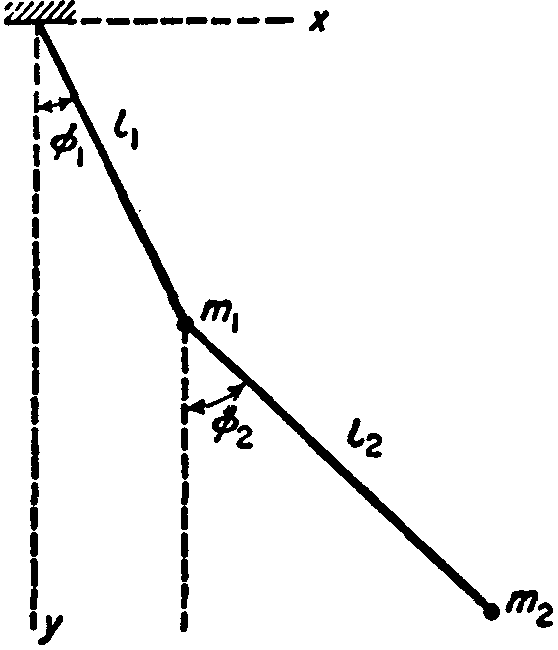
\includegraphics[width=0.75\textwidth]{landauS52_fig1.png}
%			\end{minipage}
%

\end{enumerate}
\end{document}
